% !TEX encoding = UTF-8
% !TEX TS-program = pdflatex
% !TEX root = ../tesi.tex

%**************************************************************
\chapter{Analisi dei requisiti}
\label{cap:analisi-requisiti}
%**************************************************************

\intro{In questo capitolo vengono descritte le funzionalità che il prodotto deve offrire elencando i casi d’uso e i requisiti individuati.}\\

\section{Casi d'uso}

Per lo studio dei casi di utilizzo del prodotto sono stati creati dei diagrammi.
I diagrammi dei casi d'uso\footcite{site:UseCase} (\textbf{UC}) sono diagrammi di tipo \gls{umlg} dedicati alla descrizione delle funzioni o servizi offerti da un sistema, così come sono percepiti e utilizzati dagli attori che interagiscono col sistema stesso.

\subsection{Attori principali}
Gli attori principali individuati sono i seguenti:
\begin{itemize}
    \item \textbf{Utente non autenticato}: indica l'utente che non ha effettuato l'autenticazione attraverso la procedura di login. Questo attore non deve avere la possibilità di accedere agli strumenti di voto e a quelli di monitoraggio della piattaforma;
    \item \textbf{Elettore}: indica l'utente che ha effettuato l'accesso alla piattaforma con un profilo da elettore e deve poter accedere agli strumenti di voto;
    \item \textbf{Amministratore}: indica l'utente che ha effettuato l'accesso alla piattaforma con un profilo da amministratore e deve poter accedere agli strumenti di monitoraggio delle votazioni.
\end{itemize}

\subsection{Elenco dei casi d'uso}

\begin{figure}[h!] 
    \centering 
    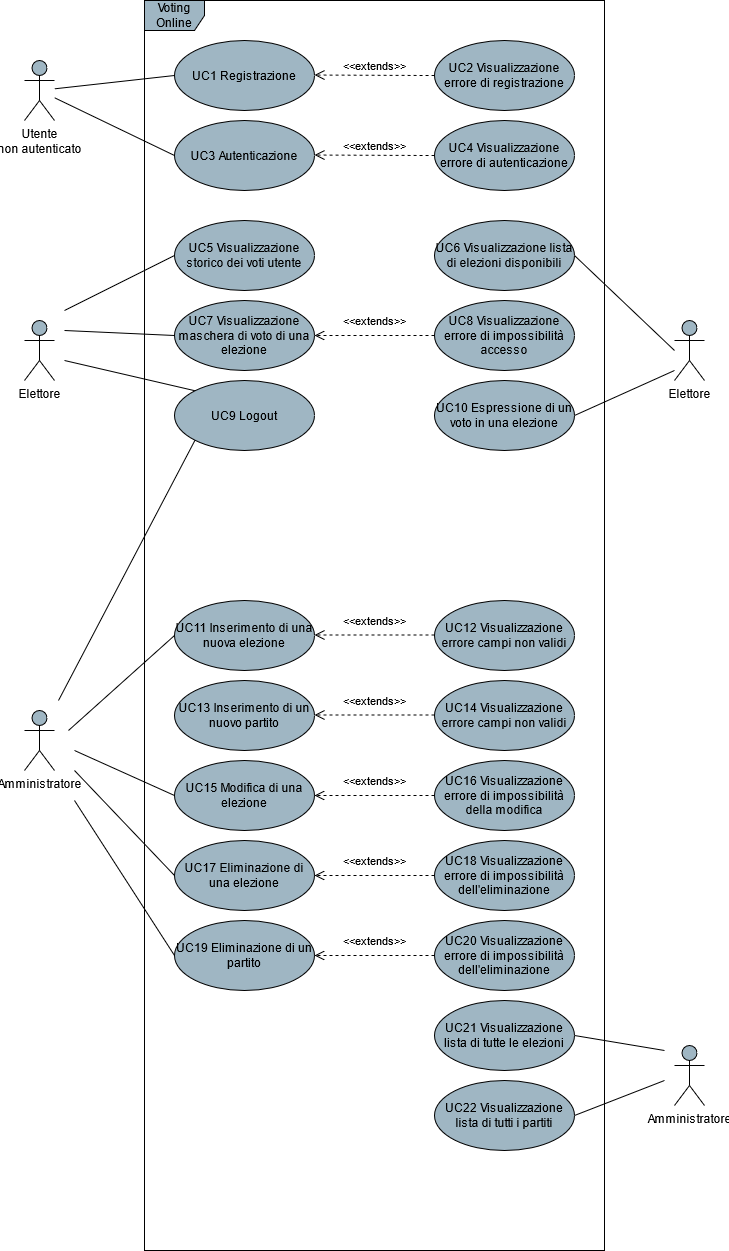
\includegraphics[width=0.9\columnwidth]{immagini/cap3/SchemaGenerale.png}
    \caption{Scenario principale}
\end{figure}

\clearpage

% ----------------------------------- UC1 ----------------------------------------------
\begin{usecase}{1}{Registrazione}
\usecaseactors{Utente non autenticato}
\usecasepre{L’utente non autenticato è all'interno della pagina di registrazione}
\usecasedesc{Viene effettuata la registrazione di un elettore nel sistema, inserendo i propri dati personali nella pagina dedicata}
\usecasescenario{L’utente non autenticato accede alla pagina di registrazione, il sistema rende disponibili i campi da compilare, l’utente inserisce l'indirizzo email [\textbf{UC1.1}], l'username [\textbf{UC1.2}], la password [\textbf{UC1.3}] e procede infine a confermare la registrazione}
\usecasepost{La registrazione nel sistema è avvenuta con successo} \\
\textbf{Estensioni:}
    \begin{enumerate}
        \item \textbf{UC2}: se i campi non sono validi o l'email è già stata utilizzata nel sistema, viene mostrato un errore di registrazione all'utente non autenticato che potrà provare nuovamente a ripetere la procedura.
    \end{enumerate}
\end{usecase}

\begin{figure}[!h] 
    \centering 
    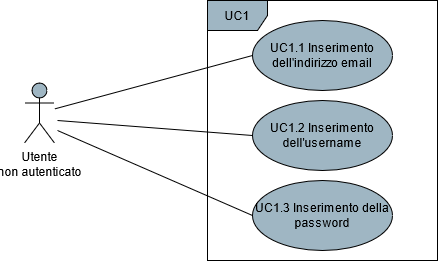
\includegraphics[width=0.9\columnwidth]{immagini/cap3/UC1.png} 
    \caption{Use Case - UC1: Registrazione}
\end{figure}

\begin{usecase}{1.1}{Inserimento dell'indirizzo email}
\usecaseactors{Utente non autenticato}
\usecasepre{Il campo “email” risulta vuoto}
\usecasedesc{L'utente deve compilare il campo “email” per procedere alla registrazione}
\usecasescenario{L'utente inserisce il suo indirizzo email nell'apposito campo}
\usecasepost{il campo “email” è stato compilato}
\end{usecase} \\ \\

\begin{usecase}{1.2}{Inserimento dell'username}
\usecaseactors{Utente non autenticato}
\usecasepre{Il campo “username” risulta vuoto}
\usecasedesc{L'utente deve compilare il campo “username” per procedere alla registrazione}
\usecasescenario{L'utente inserisce l'username desiderato nell'apposito campo}
\usecasepost{il campo “username” è stato compilato}
\end{usecase}

\begin{usecase}{1.3}{Inserimento della password}
\usecaseactors{Utente non autenticato}
\usecasepre{Il campo “password” risulta vuoto}
\usecasedesc{L'utente deve compilare il campo “password” per procedere alla registrazione}
\usecasescenario{L'utente inserisce la password desiderata nell'apposito campo}
\usecasepost{il campo “password” è stato compilato}
\end{usecase}

% ----------------------------------- UC2 ----------------------------------------------
\begin{usecase}{2}{Visualizzazione errore di registrazione}
\usecaseactors{Utente non autenticato}
\usecasepre{L'utente non autenticato ha inserito i campi ed ha provato ad effettuare
la registrazione}
\usecasedesc{L'utente non autenticato visualizza un errore riguardante i campi di registrazione che ha inserito} Questi errori possono essere:
    \begin{itemize}
        \item \textbf{campo non valido}: un campo risulta vuoto o con caratteri non validi;
        \item \textbf{email già utilizzata}: l'email è già stata utilizzata da un altro elettore.
    \end{itemize}
\usecasescenario{Il sistema riconosce uno o più errori nei campi inseriti dall'utente e vengono visualizzati nella pagina di registrazione}
\usecasepost{Viene visualizzato un messaggio di errore nella pagina di registrazione
e l’utente non risulta autenticato nel sistema} \\
\end{usecase}

% ----------------------------------- UC3 ----------------------------------------------
\begin{usecase}{3}{Autenticazione}
\usecaseactors{Utente non autenticato}
\usecasepre{L’utente non autenticato è all'interno della pagina di autenticazione}
\usecasedesc{L'utente non autenticato, inserendo le proprie credenziali, viene autenticato alla piattaforma}
\usecasescenario{L’utente non autenticato accede alla pagina di autenticazione, il sistema rende disponibili i campi da compilare, l’utente inserisce l'indirizzo email [\textbf{UC3.1}], la password [\textbf{UC3.2}] e procede infine inviando la richiesta}
\usecasepost{L'utente viene autenticato come elettore o amministratore dal sistema} \\
\textbf{Estensioni:}
    \begin{enumerate}
        \item \textbf{UC4}: se le credenziali inserite non vengono riconosciute dal sistema viene visualizzato un messaggio che informa l'utente dell'errore.
    \end{enumerate}
\end{usecase}

\begin{figure}[!h] 
    \centering 
    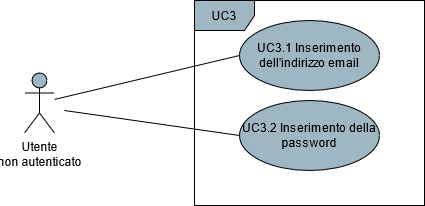
\includegraphics[width=0.9\columnwidth]{immagini/cap3/UC3.png} 
    \caption{Use Case - UC3: Autenticazione}
\end{figure}

\begin{usecase}{3.1}{Inserimento dell'indirizzo email}
\usecaseactors{Utente non autenticato}
\usecasepre{Il campo “email” risulta vuoto}
\usecasedesc{L'utente deve compilare il campo “email” per procedere all'autenticazione}
\usecasescenario{L'utente inserisce il proprio indirizzo email nell'apposito campo}
\usecasepost{il campo “email” è stato compilato}
\end{usecase}

\begin{usecase}{3.2}{Inserimento della password}
\usecaseactors{Utente non autenticato}
\usecasepre{Il campo “password” risulta vuoto}
\usecasedesc{L'utente deve compilare il campo “password” per procedere all'autenticazione}
\usecasescenario{L'utente inserisce la propria password nell'apposito campo}
\usecasepost{il campo “password” è stato compilato}
\end{usecase} \\

% ----------------------------------- UC4 ----------------------------------------------
\begin{usecase}{4}{Visualizzazione errore di autenticazione}
\usecaseactors{Utente non autenticato}
\usecasepre{L'utente non autenticato ha inserito i campi ed ha provato ad effettuare
l'autenticazione}
\usecasedesc{L'utente non autenticato visualizza un messaggio di errore che lo informa che i dati da lui inseriti durante il login non sono riconosciuti dal sistema}
\usecasescenario{:L'utente tenta di effettuare il login usando credenziali non presenti nel sistema}
\usecasepost{Viene visualizzato un messaggio di errore nella pagina di autenticazione
e l’utente non risulta autenticato nel sistema} \\
\end{usecase}

% ----------------------------------- UC5 ----------------------------------------------
\begin{usecase}{5}{Visualizzazione storico dei voti dei voti dell'utente}
\usecaseactors{Elettore}
\usecasepre{L’elettore è all'interno della pagina corrispondente alla sua dashboard personale}
\usecasedesc{L'elettore può visualizzare, nel caso abbia partecipato ad almeno un'elezione, lo storico dei propri voti}
\usecasescenario{L’elettore può visualizzare lo storico dei propri voti nella forma di una lista di singole votazioni passate [\textbf{UC5.1}]}
\usecasepost{L'elettore visualizza lo storico dei voti}
\end{usecase}

\begin{figure}[!h] 
    \centering 
    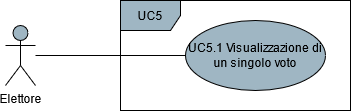
\includegraphics[width=0.9\columnwidth]{immagini/cap3/UC5.png} 
    \caption{Use Case - UC5: Visualizzazione storico dei voti dei voti dell'utente}
\end{figure}

\begin{usecase}{5.1}{Visualizzazione di un singolo voto}
\usecaseactors{Elettore}
\usecasepre{L’elettore è all'interno della pagina corrispondente alla sua dashboard personale}
\usecasedesc{L'elettore può visualizzare le informazioni corrispondenti ad un singolo voto appartenente al suo storico}
\usecasescenario{L'elettore visualizza le seguenti informazioni caratterizzanti di un voto appartenente al suo storico: il nome dell'elezione, la data di inizio e di fine dell'elezione, di espressione del voto, il partito e il candidato votato}
\usecasepost{L'elettore visualizza tutti i dati che caratterizzano un suo voto passato}
\end{usecase}

% ----------------------------------- UC6 ----------------------------------------------
\begin{usecase}{6}{Visualizzazione lista delle elezioni disponibili}
\usecaseactors{Elettore}
\usecasepre{L’elettore è all'interno della pagina corrispondente alla sua dashboard personale}
\usecasedesc{L'elettore può visualizzare, nel caso sia presente almeno un'elezione aperta nella data corrente, un elenco di elezioni}
\usecasescenario{L’elettore può visualizzare le elezioni disponibili nella forma di una lista di singole votazioni [\textbf{UC6.1}]}
\usecasepost{L'elettore visualizza le elezioni disponibili nella dashboard personale}
\end{usecase}

\begin{figure}[!h] 
    \centering 
    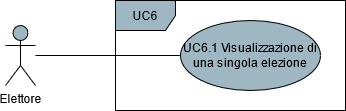
\includegraphics[width=0.9\columnwidth]{immagini/cap3/UC6.png} 
    \caption{Use Case - UC6: Visualizzazione lista delle elezioni disponibili}
\end{figure}

\begin{usecase}{6.1}{Visualizzazione di una singola elezione}
\usecaseactors{Elettore}
\usecasepre{L’elettore è all'interno della pagina corrispondente alla sua dashboard personale}
\usecasedesc{L'elettore può visualizzare le informazioni corrispondenti ad una singola elezione presente nell'elenco delle elezioni disponibili}
\usecasescenario{L'elettore visualizza le seguenti informazioni caratterizzanti di un'elezione disponibile: il nome, la tipologia, la data di inizio e di fine della votazione}
\usecasepost{L'elettore visualizza tutti i dati che caratterizzano una singola elezione disponibile}
\end{usecase}

% ----------------------------------- UC7 ----------------------------------------------
\begin{usecase}{7}{Visualizzazione maschera di voto di una elezione}
\usecaseactors{Elettore}
\usecasepre{L’elettore visualizza l'elenco delle elezioni disponibili ed è presente almeno una voce nella lista}
\usecasedesc{L'elettore accede alla maschera di voto per esprimere la propria preferenza cliccando su un'elezione disponibile, rispetto alla quale visualizzerà le informazioni nececessarie per procedere alla votazione}
\usecasescenario{L’elettore, cliccando su una delle elezioni disponibili nella lista [\textbf{UC6}], accede alla maschera di voto di tale elezione, della quale visualizza il relativo nome, le istruzioni per esprimere la propria preferenza con successo e la lista dei partiti partecipanti [\textbf{UC7.1}]}
\usecasepost{L'elettore visualizza le informazioni necessarie per esprimere il proprio voto nell'apposita pagina}
\textbf{Estensioni:}
    \begin{enumerate}
        \item \textbf{UC8}: se si clicca su un'elezione per la quale l'elettore ha già espresso una preferenza viene visualizzato un messaggio che avvisa l'utente dell'errore.
    \end{enumerate}
\end{usecase}

\begin{figure}[!h] 
    \centering 
    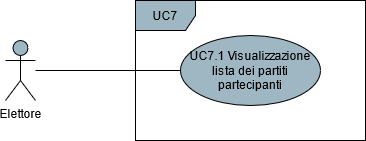
\includegraphics[width=0.9\columnwidth]{immagini/cap3/UC7.png} 
    \caption{Use Case - UC7: Visualizzazione maschera di voto di una elezione}
\end{figure}

\begin{usecase}{7.1}{Visualizzazione lista dei partiti partecipanti}
\usecaseactors{Elettore}
\usecasepre{L’elettore è all'interno della pagina corrispondente alla maschera di voto per una elezione}
\usecasedesc{L'elettore può visualizzare, nel caso sia presente almeno un partito partecipante, una lista di partiti}
\usecasescenario{L’elettore può visualizzare i partiti partecipanti nella forma di una lista di singoli partiti [\textbf{UC7.1.1}]}
\usecasepost{L'elettore visualizza tutti i partiti partecipanti che possono essere votati nella maschera di voto relativa ad una specifica elezione}
\end{usecase} \\

\begin{figure}[!h] 
    \centering 
    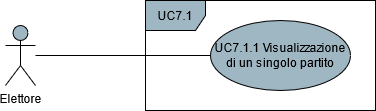
\includegraphics[width=0.9\columnwidth]{immagini/cap3/UC7_1.png} 
    \caption{Use Case - UC7.1: Visualizzazione lista dei partiti partecipanti}
\end{figure}

\begin{usecase}{7.1.1}{Visualizzazione di un singolo partito}
\usecaseactors{Elettore}
\usecasepre{L’elettore è all'interno della pagina corrispondente alla maschera di voto per una elezione e sta visualizzando la lista dei partiti partecipanti}
\usecasedesc{L'elettore può visualizzare le informazioni corrispondenti ad un singolo partito presente nell'elenco dei partiti partecipanti}
\usecasescenario{L'elettore visualizza le seguenti informazioni caratterizzanti del partito partecipante: il logo, il nome e il nominativo del candidato associato al partito}
\usecasepost{L'elettore visualizza tutti i dati che caratterizzano un singolo partito partecipante all'elezione}
\end{usecase}

% ----------------------------------- UC8 ----------------------------------------------
\begin{usecase}{8}{Visualizzazione errore di impossibilità di accesso all'elezione}
\usecaseactors{Elettore}
\usecasepre{L’elettore visualizza l'elenco delle elezioni disponibili ed ha provato a cliccare su una delle voci presenti nella lista}
\usecasedesc{L'elettore visualizza un messaggio di errore riguardante l'impossibilità di accedere alla maschera di voto relativa all'elezione selezionata. Questo errore indica che è stata già effettuata una preferenza per questa elezione}
\usecasescenario{Il sistema riconosce un errore al tentativo di accesso da parte dell'elettore ad un'elezione e viene visualizzato il relativo messaggio di errore nella dashboard personale}
\usecasepost{Viene visualizzato un messaggio di errore nella dashboard personale dell'elettore e quest'ultimo non ha la possibilità di accedere alla maschera di voto relativa all'elezione selezionata} \\
\end{usecase}

% ----------------------------------- UC9 ----------------------------------------------
\begin{usecase}{9}{Logout}
\usecaseactors{Elettore, Amministratore}
\usecasepre{L'utente, che ha precedentemente effettuato la procedura di login, è attualmente autenticato nella piattaforma}
\usecasedesc{Viene effettuato il logout di un'utente autenticato, che può essere un elettore o amministratore}
\usecasescenario{L'utente richiede il logout tramite un bottone dedicato}
\usecasepost{L'utente non è più autenticato nel sistema} \\ \\
\end{usecase}

% ----------------------------------- UC10 ----------------------------------------------
\begin{usecase}{10}{Espressione di un voto in un'elezione}
\usecaseactors{Elettore}
\usecasepre{L’elettore si trova nella pagina relativa alla maschera di voto di una specifica elezione}
\usecasedesc{L'elettore può esprimere il proprio voto in una determinata elezione selezionando il partito desiderato e confermando infine la propria scelta}
\usecasescenario{L'elettore, visualizzando le informazioni contenute nella maschera di voto [\textbf{UC7}] dell'elezione in questione, può procedere ad esprimere la propria preferenza selezionando uno tra i partiti partecipanti [\textbf{UC10.1}] e confermando successivamente la propria decisione [\textbf{UC10.2}]}
\usecasepost{L'elettore ha votato per un partito partecipante ad una specifica elezione}
\end{usecase}

\begin{figure}[!h] 
    \centering
    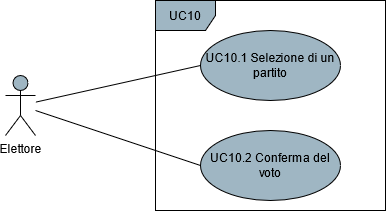
\includegraphics[width=0.9\columnwidth]{immagini/cap3/UC10.png} 
    \caption{Use Case - UC10: Espressione di un voto in un'elezione}
\end{figure}

\begin{usecase}{10.1}{Selezione di un partito}
\usecaseactors{Elettore}
\usecasepre{L’elettore si trova nella pagina relativa alla maschera di voto di una specifica elezione}
\usecasedesc{L'elettore deve selezionare esattamente un partito dalla lista dei partiti partecipanti per poter continuare con la procedura di voto}
\usecasescenario{L'elettore, visualizzando la lista di partiti partecipanti contenuta nella maschera di voto [\textbf{UC7.1}] dell'elezione in questione, deve selezionare esattamente uno tra i partiti partecipanti per esprimere la propria preferenza}
\usecasepost{L'elettore ha selezionato un partito partecipante all'elezione in questione} \\ \\
\end{usecase}

\begin{usecase}{10.2}{Conferma del voto}
\usecaseactors{Elettore}
\usecasepre{L’elettore si trova nella pagina relativa alla maschera di voto di una specifica elezione ed ha selezionato un partito partecipante}
\usecasedesc{L'elettore deve confermare il partito scelto come preferenza per concludere la votazione}
\usecasescenario{L'elettore, dopo aver selezionato un partito partecipante come preferenza [\textbf{UC10.1}], deve cliccare sull'apposito pulsante per richiedere la conclusione della votazione e, visualizzando un apposito riquadro di riepilogo, deve confermare la propria decisione per concludere la procedura di voto}
\usecasepost{L'elettore ha confermato la preferenza del partito partecipante scelto all'elezione in questione}
\end{usecase}

% ----------------------------------- UC11 ----------------------------------------------
\begin{usecase}{11}{Inserimento di una nuova elezione}
\usecaseactors{Amministratore}
\usecasepre{L’amministratore si trova nella pagina corrispondente alla admin dashboard}
\usecasedesc{L'amministratore può inserire una nuova elezione nella piattaforma inserendo gli appositi dati}
\usecasescenario{L'amministratore per inserire una nuova elezione deve compilare i campi dati in modo da descriverne le seguenti informazioni: il nome [\textbf{UC11.1}], la tipologia [\textbf{UC11.2}], la data di inizio [\textbf{UC11.3}] e di fine [\textbf{UC11.4}]. E' necessario, infine, che vengano selezionati i partiti partecipanti da un apposito elenco [\textbf{UC11.5}]}
\usecasepost{L'amministratore ha inserito una nuova elezione nel sistema con successo} \\
\textbf{Estensioni:}
    \begin{enumerate}
        \item \textbf{UC12}: se i campi non sono validi viene mostrato un errore di inserimento all'amministratore che potrà provare nuovamente a ripetere la procedura modificando i campi che hanno causato l'errore.
    \end{enumerate}
\end{usecase}

\begin{figure}[!h] 
    \centering
    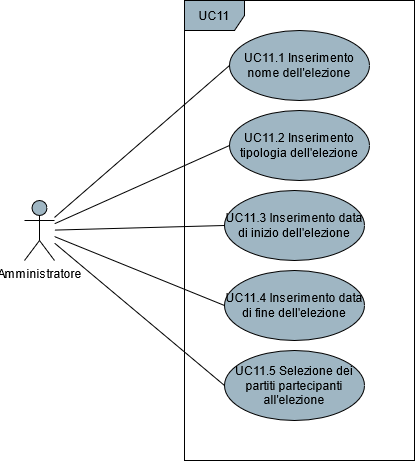
\includegraphics[width=0.9\columnwidth]{immagini/cap3/UC11.png} 
    \caption{Use Case - UC11: Inserimento di una nuova elezione}
\end{figure}

\begin{usecase}{11.1}{Inserimento del nome}
\usecaseactors{Amministratore}
\usecasepre{Il campo “nome” risulta vuoto}
\usecasedesc{L'amministratore deve compilare il campo “nome” per procedere all'inserimento}
\usecasescenario{L'amministratore inserisce il nome dell'elezione nell'apposito campo}
\usecasepost{il campo “nome” è stato compilato}
\end{usecase}

\begin{usecase}{11.2}{Inserimento della tipologia}
\usecaseactors{Amministratore}
\usecasepre{Il campo “tipologia” risulta vuoto}
\usecasedesc{L'amministratore deve compilare il campo “tipologia” per procedere all'inserimento}
\usecasescenario{L'amministratore inserisce la tipologia dell'elezione nell'apposito campo}
\usecasepost{il campo “tipologia” è stato compilato}
\end{usecase}

\begin{usecase}{11.3}{Inserimento della data di inizio}
\usecaseactors{Amministratore}
\usecasepre{Il campo “data di inizio” risulta vuoto}
\usecasedesc{L'amministratore deve compilare il campo “data di inizio” per procedere all'inserimento}
\usecasescenario{L'amministratore inserisce la data di inizio dell'elezione nell'apposito campo}
\usecasepost{il campo “data di inizio” è stato compilato}
\end{usecase}

\begin{usecase}{11.4}{Inserimento della data di fine}
\usecaseactors{Amministratore}
\usecasepre{Il campo “data di fine” risulta vuoto}
\usecasedesc{L'amministratore deve compilare il campo “data di fine” per procedere all'inserimento}
\usecasescenario{L'amministratore inserisce la data di fine dell'elezione nell'apposito campo}
\usecasepost{il campo “data di fine” è stato compilato}
\end{usecase}

\begin{usecase}{11.5}{Selezione dei partiti partecipanti all'elezione}
\usecaseactors{Amministratore}
\usecasepre{Nessun partito risulta selezionato nell'elenco dei partiti partecipanti}
\usecasedesc{L'amministratore può decidere di selezionare nessuno o tutti i partiti presenti nel sistema in modo da renderli partecipanti all'elezione. La selezione dei partiti partecipanti è modificabile in seguito utilizzando la funzionalità di modifica dell'elezione [\textbf{UC15}]}
\usecasescenario{L'amministratore decide quali partiti aggiungere all'elezione in questione selezionandoli nell'apposito elenco che contiene tutti i partiti presenti nella piattaforma}
\usecasepost{L'elenco dei partiti partecipanti è stato compilato da parte dell'amministratore}
\end{usecase}

% ----------------------------------- UC12 ----------------------------------------------
\begin{usecase}{12}{Visualizzazione errore per campi non validi}
\usecaseactors{Amministratore}
\usecasepre{L'amministratore ha compilato i campi ed ha provato ad effettuare l'inserimento di una nuova elezione}
\usecasedesc{L'amministratore visualizza un errore riguardante uno o più campi che ha compilato e che risultano invalidi perchè vuoti o perchè c'è un errore nella formattazione del contenuto}
\usecasescenario{Il sistema riconosce uno o più errori nei campi inseriti dall'amministratore e vengono visualizzati nell'apposita form di inserimento}
\usecasepost{Viene visualizzato un messaggio di errore nella form e la nuova elezione non risulta inserita nel sistema} \\
\end{usecase}

% ----------------------------------- UC13 ----------------------------------------------
\begin{usecase}{13}{Inserimento di un nuovo partito}
\usecasepre{L’amministratore si trova nella pagina corrispondente alla admin dashboard}
\usecasedesc{L'amministratore può inserire un nuovo partito nella piattaforma inserendo gli appositi dati}
\usecasescenario{L'amministratore per inserire un nuovo partito deve compilare i campi dati in modo da descriverne le seguenti caratteristiche: il nome [\textbf{UC13.1}] e il nominativo del candidato [\textbf{UC13.2}]. E' necessario, infine, che venga inserito il logo del partito in formato immagine (PNG/JPEG) [\textbf{UC13.3}]}
\usecasepost{L'amministratore ha inserito un nuovo partito nel sistema con successo} \\
\textbf{Estensioni:}
    \begin{enumerate}
        \item \textbf{UC14}: se i campi non sono validi viene mostrato un errore di inserimento all'amministratore che potrà provare nuovamente a ripetere la procedura modificando i campi che hanno causato l'errore.
    \end{enumerate}
\end{usecase}

\begin{figure}[!h] 
    \centering
    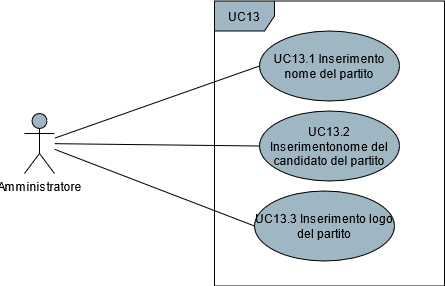
\includegraphics[width=0.9\columnwidth]{immagini/cap3/UC13.png} 
    \caption{Use Case - UC13: Inserimento di un nuovo partito}
\end{figure}

\begin{usecase}{13.1}{Inserimento del nome}
\usecaseactors{Amministratore}
\usecasepre{Il campo “nome” risulta vuoto}
\usecasedesc{L'amministratore deve compilare il campo “nome” per procedere all'inserimento}
\usecasescenario{L'amministratore inserisce il nome del partito nell'apposito campo}
\usecasepost{il campo “nome” è stato compilato}
\end{usecase}

\begin{usecase}{13.2}{Inserimento del candidato}
\usecaseactors{Amministratore}
\usecasepre{Il campo “candidato” risulta vuoto}
\usecasedesc{L'amministratore deve compilare il campo “candidato” inserendo il nominativo del candidato per il partito in modo da procedere all'inserimento}
\usecasescenario{L'amministratore inserisce il nominativo del candidato del partito nell'apposito campo}
\usecasepost{il campo “candidato” è stato compilato}
\end{usecase}

\begin{usecase}{13.3}{Inserimento del logo}
\usecaseactors{Amministratore}
\usecasepre{Il campo nel quale inserire il logo del partito risulta vuoto}
\usecasedesc{L'amministratore deve inserire il logo del partito in formato immagine (PNG/JPEG) per procedere all'inserimento}
\usecasescenario{L'amministratore inserisce il logo del partito nell'apposito campo}
\usecasepost{Il logo del partito è stato inserito nell'apposito campo}
\end{usecase}

% ----------------------------------- UC14 ----------------------------------------------
\begin{usecase}{14}{Visualizzazione errore per campi non validi}
\usecaseactors{Amministratore}
\usecasepre{L'amministratore ha compilato i campi ed ha provato ad effettuare l'inserimento di un nuovo partito}
\usecasedesc{L'amministratore visualizza un errore riguardante uno o più campi che ha compilato e che risultano invalidi perchè vuoti o perchè c'è un errore nella formattazione del contenuto}
\usecasescenario{Il sistema riconosce uno o più errori nei campi inseriti dall'amministratore e vengono visualizzati nell'apposita form di inserimento}
\usecasepost{Viene visualizzato un messaggio di errore nella form e il nuovo partito non risulta inserito nel sistema}
\end{usecase}

% ----------------------------------- UC15 ----------------------------------------------
\begin{usecase}{15}{Modifica di una elezione}
\usecaseactors{Amministratore}
\usecasepre{L’amministratore si trova nella pagina corrispondente alla admin dashboard e visualizza le informazioni di dettaglio di un'elezione}
\usecasedesc{L'amministratore può modificare un'elezione presente nella piattaforma compilando gli appositi campi dati}
\usecasescenario{L'amministratore per modificare un'elezione esistente deve, rendendo editabili le sue informazioni attraverso l'apposito pulsante, compilare i campi dati in modo da descrivere almeno una delle seguenti informazioni: il nome [\textbf{UC15.1}], la tipologia [\textbf{UC15.2}], la data di inizio [\textbf{UC15.3}] e di fine [\textbf{UC15.4}]. E' possibile, inoltre, modificare i partiti partecipanti alterando le voci selezionate di un apposito elenco [\textbf{UC15.5}] e, infine, la modifica deve essere confermata da un apposito pulsante}
\usecasepost{L'amministratore ha modificato un'elezione presente nel sistema con successo} \\
\textbf{Estensioni:}
    \begin{enumerate}
        \item \textbf{UC16}: nel caso in cui un'elezione risulti cominciata o già terminata non è possibile modificarla, verrà quindi mostrato un messaggio esplicativo all'amministratore, il quale non potrà procedere con la modifica.
    \end{enumerate}
\end{usecase}

\begin{figure}[!h] 
    \centering
    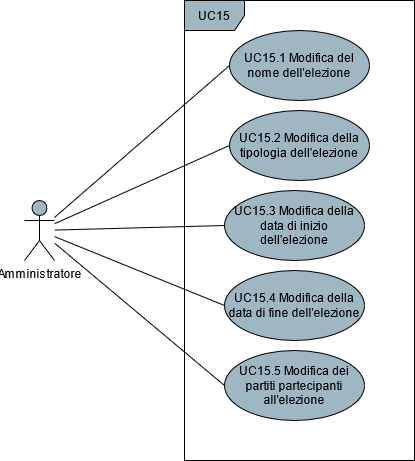
\includegraphics[width=0.9\columnwidth]{immagini/cap3/UC15.png} 
    \caption{Use Case - UC15: Modifica di una elezione}
\end{figure}

\begin{usecase}{15.1}{Modifica del nome}
\usecaseactors{Amministratore}
\usecasepre{Il campo “nome” risulta occupato dall'informazione attuale dell'elezione}
\usecasedesc{L'amministratore può compilare il campo “nome” per procedere alla modifica di tale informazione}
\usecasescenario{L'amministratore inserisce il nuovo nome dell'elezione nell'apposito campo}
\usecasepost{il campo “nome” è stato modificato}
\end{usecase}

\begin{usecase}{15.2}{Modifica della tipologia}
\usecaseactors{Amministratore}
\usecasepre{Il campo “tipologia” risulta occupato dall'informazione attuale dell'elezione}
\usecasedesc{L'amministratore può compilare il campo “tipologia” per procedere alla modifica di tale informazione}
\usecasescenario{L'amministratore inserisce la nuova tipologia dell'elezione nell'apposito campo}
\usecasepost{il campo “tipologia” è stato modificato}
\end{usecase}

\begin{usecase}{15.3}{Modifica della data di inizio}
\usecaseactors{Amministratore}
\usecasepre{Il campo “data di inizio” risulta occupato dall'informazione attuale dell'elezione}
\usecasedesc{L'amministratore può compilare il campo “data di inizio” per procedere alla modifica di tale informazione}
\usecasescenario{L'amministratore inserisce la nuova data di inizio dell'elezione nell'apposito campo}
\usecasepost{il campo “data di inizio” è stato modificato}
\end{usecase}

\begin{usecase}{15.4}{Modifica della data di fine}
\usecaseactors{Amministratore}
\usecasepre{Il campo “data di fine” risulta occupato dall'informazione attuale dell'elezione}
\usecasedesc{L'amministratore può compilare il campo “data di fine” per procedere alla modifica di tale informazione}
\usecasescenario{L'amministratore inserisce la nuova data di fine dell'elezione nell'apposito campo}
\usecasepost{il campo “data di fine” è stato modificato}
\end{usecase}

\begin{usecase}{15.5}{Modifica dei partiti partecipanti all'elezione}
\usecaseactors{Amministratore}
\usecasepre{L'elenco dei partiti partecipanti contiene le informazioni attuali riguardo ai partiti}
\usecasedesc{L'amministratore può decidere di modificare l'elenco selezionando nessuno o tutti i partiti presenti nel sistema in modo da renderli partecipanti all'elezione. La selezione dei partiti partecipanti è modificabile finché non arriva la data di inizio dell'elezione}
\usecasescenario{L'amministratore decide quali partiti aggiungere o rimuovere dall'elezione in questione selezionandoli nell'apposito elenco che contiene tutti i partiti presenti nella piattaforma}
\usecasepost{L'elenco dei partiti partecipanti è stato modificato da parte dell'amministratore}
\end{usecase}

% ----------------------------------- UC16 ----------------------------------------------
\begin{usecase}{16}{Visualizzazione errore per impossibilità della modifica}
\usecaseactors{Amministratore}
\usecasepre{L'amministratore visualizza le informazioni riguardanti un'elezione già cominciata o conclusa ed ha provato a cliccare sul pulsante per abilitare la loro modifica}
\usecasedesc{Viene mostrato all'amministratore un messaggio che indica che non è possibile modificare un'elezione già cominciata o conclusa}
\usecasescenario{Il sistema mostra un messaggio esplicativo dell'errore all'amministratore}
\usecasepost{Viene visualizzato un messaggio di errore nella admin dashboard e non viene permessa la modifica dell'elezione all'amministratore} \\
\end{usecase}

% ----------------------------------- UC17 ----------------------------------------------
\begin{usecase}{17}{Eliminazione di una elezione}
\usecaseactors{Amministratore}
\usecasepre{L’amministratore si trova nella pagina corrispondente alla admin dashboard e visualizza le informazioni di dettaglio di un'elezione}
\usecasedesc{L'amministratore può eliminare un'elezione presente nella piattaforma cliccando l'apposito pulsante}
\usecasescenario{L'amministratore per eliminare un'elezione esistente deve premere l'apposito pulsante situato contestualmente alle informazioni dell'elezione stessa}
\usecasepost{L'amministratore ha eliminato un'elezione presente nel sistema con successo} \\
\textbf{Estensioni:}
    \begin{enumerate}
        \item \textbf{UC18}: nel caso in cui un'elezione risulti cominciata o già terminata non è possibile eliminarla, verrà quindi mostrato un messaggio esplicativo all'amministratore, il quale non potrà procedere con l'eliminazione.
    \end{enumerate}
\end{usecase}

% ----------------------------------- UC18 ----------------------------------------------
\begin{usecase}{18}{Visualizzazione errore per impossibilità dell'eliminazione}
\usecaseactors{Amministratore}
\usecasepre{L'amministratore visualizza le informazioni riguardanti un'elezione già cominciata o conclusa ed ha provato a cliccare sul pulsante per eliminarla}
\usecasedesc{Viene mostrato all'amministratore un messaggio che indica che non è possibile eliminare un'elezione già cominciata o conclusa}
\usecasescenario{Il sistema mostra un messaggio esplicativo dell'errore all'amministratore}
\usecasepost{Viene visualizzato un messaggio di errore nella admin dashboard e non viene permessa l'eliminazione dell'elezione all'amministratore} \\
\end{usecase}

% ----------------------------------- UC19 ----------------------------------------------
\begin{usecase}{19}{Eliminazione di un partito}
\usecaseactors{Amministratore}
\usecasepre{L’amministratore si trova nella pagina corrispondente alla admin dashboard e visualizza le informazioni di dettaglio di un partito}
\usecasedesc{L'amministratore può eliminare un partito presente nella piattaforma cliccando l'apposito pulsante}
\usecasescenario{L'amministratore per eliminare un partito esistente deve premere l'apposito pulsante situato contestualmente alle informazioni del partito stesso}
\usecasepost{L'amministratore ha eliminato un partito dal sistema con successo} \\
\textbf{Estensioni:}
    \begin{enumerate}
        \item \textbf{UC20}: nel caso in cui un partito risulti presente in un'elezione già cominciata o terminata non è possibile eliminarlo, verrà quindi mostrato un messaggio esplicativo all'amministratore, il quale non potrà procedere con l'eliminazione.
    \end{enumerate}
\end{usecase}

% ----------------------------------- UC20 ----------------------------------------------
\begin{usecase}{20}{Visualizzazione errore per impossibilità dell'eliminazione}
\usecaseactors{Amministratore}
\usecasepre{L'amministratore visualizza le informazioni riguardanti un partito partecipante in un'elezione già cominciata o conclusa ed ha provato a cliccare sul pulsante per eliminarlo}
\usecasedesc{Viene mostrato all'amministratore un messaggio che indica che non è possibile eliminare un partito facente parte di un'elezione già cominciata o conclusa}
\usecasescenario{Il sistema mostra un messaggio esplicativo dell'errore all'amministratore}
\usecasepost{Viene visualizzato un messaggio di errore nella admin dashboard e non viene permessa l'eliminazione del partito all'amministratore}
\end{usecase}

% ----------------------------------- UC21 ----------------------------------------------
\begin{usecase}{21}{Visualizzazione lista di tutte le elezioni}
\usecaseactors{Amministratore}
\usecasepre{L’amministratore è all'interno della pagina corrispondente all'admin dashboard}
\usecasedesc{L'amministratore può visualizzare, nel caso sia stata inserita nella piattaforma almeno un'elezione, un elenco di elezioni}
\usecasescenario{L’amministratore può visualizzare tutte le elezioni precedentemente inserite nella piattaforma con la forma di una lista di singole votazioni [\textbf{UC21.1}]}
\usecasepost{L'amministratore visualizza le elezioni presenti nella piattaforma sulla admin dashboard}
\end{usecase}

\begin{figure}[!h] 
    \centering 
    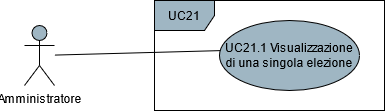
\includegraphics[width=0.9\columnwidth]{immagini/cap3/UC21.png} 
    \caption{Use Case - UC21: Visualizzazione lista di tutte le elezioni}
\end{figure}

\begin{usecase}{21.1}{Visualizzazione di una singola elezione}
\usecaseactors{Amministratore}
\usecasepre{L'amministratore è all'interno della pagina corrispondente all'admin dashboard}
\usecasedesc{L'amministratore può visualizzare le informazioni corrispondenti ad una singola elezione presente nell'elenco di tutte le elezioni}
\usecasescenario{L'amministratore visualizza le seguenti informazioni caratterizzanti di un'elezione: il nome, la tipologia, la data di inizio e di fine della votazione}
\usecasepost{L'amministratore visualizza tutti i dati che caratterizzano una singola elezione}
\end{usecase}

% ----------------------------------- UC22 ----------------------------------------------
\begin{usecase}{22}{Visualizzazione lista di tutti i partiti}
\usecaseactors{Amministratore}
\usecasepre{L’amministratore è all'interno della pagina corrispondente all'admin dashboard}
\usecasedesc{L'amministratore può visualizzare, nel caso sia stato inserito nella piattaforma almeno un partito, un elenco di partiti}
\usecasescenario{L’amministratore può visualizzare tutti i partiti precedentemente inseriti nella piattaforma con la forma di una lista di singoli partiti [\textbf{UC22.1}]}
\usecasepost{L'amministratore visualizza tutti i partiti presenti nella piattaforma sulla admin dashboard}
\end{usecase}

\begin{figure}[!h] 
    \centering 
    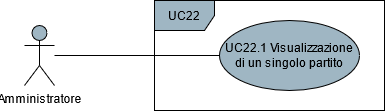
\includegraphics[width=0.9\columnwidth]{immagini/cap3/UC22.png} 
    \caption{Use Case - UC22: Visualizzazione lista di tutti i partiti}
\end{figure}

\begin{usecase}{22.1}{Visualizzazione di un singolo partito}
\usecaseactors{Amministratore}
\usecasepre{L'amministratore è all'interno della pagina corrispondente all'admin dashboard}
\usecasedesc{L'amministratore può visualizzare le informazioni che caratterizzano un singolo partito presente nell'elenco di tutti i partiti}
\usecasescenario{L'amministratore visualizza le seguenti informazioni caratterizzanti di un'elezione disponibile: il nome, il logo e il nominativo del candidato del partito}
\usecasepost{L'amministratore visualizza tutti i dati che caratterizzano un singolo partito}
\end{usecase}

% ----------------------------- TRACCIAMENTO REQUISITI --------------------------------------

\section{Tracciamento dei requisiti}

Da un'attenta analisi dei requisiti e degli use case effettuata sul progetto è stata stilata la tabella che traccia i requisiti in rapporto agli use case.\\
Sono stati individuati diversi tipi di requisiti e si è quindi fatto utilizzo di un codice identificativo per distinguerli.\\
Il codice dei requisiti è così strutturato R(F/Q/V)(N/D/O) dove:
\begin{enumerate}
	\item[R =] requisito
    \item[F =] funzionale
    \item[Q =] qualitativo
    \item[V =] di vincolo
    \item[N =] obbligatorio (necessario)
    \item[D =] desiderabile
    \item[Z =] opzionale
\end{enumerate}
Le fonti dei requisiti possono essere le seguenti:
\begin{itemize}
    \item UC[numero]: indica un caso d'uso;
    \item Committente: indica il capo progetto.
\end{itemize}
Nelle tabelle \ref{tab:requisiti-funzionali}, \ref{tab:requisiti-qualitativi} e \ref{tab:requisiti-vincolo} sono riassunti i requisiti e il loro tracciamento con gli use case delineati in fase di analisi.

\newpage

%\begin{table}%
%\caption{Tabella del tracciamento dei requisti funzionali}
%\label{tab:requisiti-funzionali}
%\begin{tabularx}{\textwidth}{lXl}
\begin{longtable}{| p{.20\textwidth} | p{.60\textwidth} | p{.20\textwidth} |}
\caption{Tabella del tracciamento dei requisti funzionali}
\label{tab:requisiti-funzionali}
\hline

\textbf{Requisito} & \textbf{Descrizione} & \textbf{Fonte}\\

\hline

RFN-1     & Il sistema deve permettere la registrazione di un nuovo elettore & UC1 \\

\hline

RFN-1.1     & Il sistema deve permettere l'inserimento dell'indirizzo email in fase di registrazione & UC1.1 \\

\hline

RFN-1.2     & Il sistema deve permettere l'inserimento dell'username in fase di registrazione & UC1.2 \\

\hline

RFN-1.3     & Il sistema deve permettere l'inserimento della password in fase di registrazione & UC1.3 \\

\hline

RFN-2     & Il sistema deve mostrare un errore nel caso in cui i campi non siano validi in fase di registrazione & UC2 \\

\hline

RFN-3     & Il sistema deve permettere l'autenticazione di un utente registrato come elettore o amministratore & UC3 \\

\hline

RFN-3.1     & Il sistema deve permettere l'inserimento dell'indirizzo email in fase di autenticazione & UC3.1 \\

\hline

RFN-3.2     & Il sistema deve permettere l'inserimento della password in fase di autenticazione & UC3.2 \\

\hline

RFN-4     & Il sistema deve mostrare un errore nel caso in cui i dati inseriti negli appositi campi non vengano riconosciuti in fase di autenticazione & UC4 \\

\hline

RFN-5     & Il sistema deve permettere di visualizzare lo storico dei voti ad un elettore & UC5 \\

\hline

RFN-5.1     & Il sistema deve permettere di visualizzare le informazioni di ogni singolo voto appartenente allo storico di un elettore & UC5.1 \\

\hline

RFN-6     & Il sistema deve permettere di visualizzare tutte le elezioni disponibili ad un elettore & UC6 \\

\hline

RFN-6.1     & Il sistema deve permettere di visualizzare le informazioni di ogni singola votazione appartenente alle elezioni disponibili di un elettore & UC6.1 \\

\hline

RFN-7     & Il sistema deve permettere di visualizzare la maschera di voto di una specifica elezione ad un elettore & UC7 \\

\hline

RFN-7.1     & Il sistema deve permettere di visualizzare la lista dei partiti partecipanti nella maschera di voto di una specifica elezione & UC7.1 \\

\hline

RFN-7.1.1     & Il sistema deve permettere di visualizzare le informazioni di ogni singolo partito partecipante nella maschera di voto di una specifica elezione & UC7.1.1 \\

\hline

RFN-8     & Il sistema deve mostrare un errore nel caso in cui l'elettore provi ad accedere alla maschera di voto di un'elezione per la quale ha già espresso il proprio voto & UC8 \\

\hline

RFN-9     & Il sistema deve permettere l'uscita dalla piattaforma da parte di un utente precedentemente auteticato come elettore o amministratore & UC9 \\

\hline

RFN-10     & Il sistema deve permettere ad un elettore l'espressione della propria preferenza all'interno della maschera di voto di una specifica elezione  & UC10 \\

\hline

RFN-10.1     & Il sistema deve permettere ad un elettore di selezionare esattamente un partito dalla lista dei partiti partecipanti nella maschera di voto  & UC10.1 \\

\hline

RFD-10.2     & Il sistema deve permettere ad un elettore di confermare la scelta del partito selezionato, visualizzando un riquadro di riepilogo  & UC10.2 \\

\hline

RFN-11     & Il sistema deve permettere ad un amministratore l'inserimento di una nuova elezione nella piattaforma  & UC11 \\

\hline

RFN-11.1     & Il sistema deve permettere ad un amministratore l'inserimento del nome in fase di inserimento di una nuova elezione  & UC11.1 \\

\hline

RFN-11.2     & Il sistema deve permettere ad un amministratore l'inserimento della tipologia in fase di inserimento di una nuova elezione  & UC11.2 \\

\hline

RFN-11.3     & Il sistema deve permettere ad un amministratore l'inserimento della data di inizio in fase di inserimento di una nuova elezione  & UC11.3 \\

\hline

RFN-11.4     & Il sistema deve permettere ad un amministratore l'inserimento della data di fine in fase di inserimento di una nuova elezione  & UC11.4 \\

\hline

RFN-11.5     & Il sistema deve permettere ad un amministratore la selezione dei partiti partecipanti, tra quelli presenti nella piattaforma, in fase di inserimento di una nuova elezione  & UC11.5 \\

\hline

RFN-12     & Il sistema deve mostrare un errore nel caso in cui i campi compilati in fase di inserimento di una nuova elezione dall'amministratore risultino invalidi perchè vuoti o con errori di formattazione del contenuto  & UC12 \\

\hline

RFN-13     & Il sistema deve permettere ad un amministratore l'inserimento di un nuovo partito nella piattaforma  & UC13 \\

\hline

RFN-13.1     & Il sistema deve permettere ad un amministratore l'inserimento del nome in fase di inserimento di un nuovo partito  & UC13.1 \\

\hline

RFN-13.2     & Il sistema deve permettere ad un amministratore l'inserimento del nominativo del candidato in fase di inserimento di un nuovo partito  & UC13.2 \\

\hline

RFN-13.3     & Il sistema deve permettere ad un amministratore l'inserimento del logo in fase di inserimento di un nuovo partito  & UC13.3 \\

\hline

RFN-14     & Il sistema deve mostrare un errore nel caso in cui i campi compilati in fase di inserimento di un nuovo partito dall'amministratore risultino invalidi perchè vuoti o con errori di formattazione del contenuto  & UC14 \\

\hline

RFN-15     & Il sistema deve permettere ad un amministratore la modifica di un'elezione presente nella piattaforma  & UC15 \\

\hline

RFN-15.1     & Il sistema deve permettere ad un amministratore l'inserimento del nuovo nome in fase di modifica di una elezione  & UC15.1 \\

\hline

RFN-15.2     & Il sistema deve permettere ad un amministratore l'inserimento della nuova tipologia in fase di modifica di una elezione  & UC15.2 \\

\hline

RFN-15.3     & Il sistema deve permettere ad un amministratore l'inserimento della nuova data di inizio in fase di modifica di una elezione  & UC15.3 \\

\hline

RFN-15.4     & Il sistema deve permettere ad un amministratore l'inserimento della nuova data di fine in fase di modifica di una elezione  & UC15.4 \\

\hline

RFN-15.5     & Il sistema deve permettere ad un amministratore l'aggiornamento dei partiti partecipanti, sempre tra quelli presenti nella piattaforma, in fase di modifica di una elezione  & UC15.5 \\

\hline

RFN-16     & Il sistema deve mostrare un errore nel caso in cui l'amministratore provi a modificare un'elezione che risulti già cominciata o terminata  & UC16 \\

\hline

RFN-17     & Il sistema deve permettere ad un amministratore l'eliminazione di un'elezione presente nella piattaforma  & UC17 \\

\hline

RFN-18     & Il sistema deve mostrare un errore nel caso in cui l'amministratore provi ad eliminare un'elezione che risulti già cominciata o terminata  & UC18 \\

\hline

RFN-19     & Il sistema deve permettere ad un amministratore l'eliminazione di un partito presente nella piattaforma  & UC19 \\

\hline

RFN-20     & Il sistema deve mostrare un errore nel caso in cui l'amministratore provi ad eliminare un partito che risulti partecipante in un'elezione già cominciata o terminata  & UC20 \\

\hline

RFN-21     & Il sistema deve permettere ad un amministratore la visualizzazione di una lista contenente tutte le elezioni presenti nella piattaforma & UC21 \\

\hline

RFN-21.1     & Il sistema deve permettere ad un amministratore di visualizzare le informazioni di ogni singola elezione appartenente alla lista di tutte le elezioni presenti nella piattaforma & UC21.1 \\

\hline

RFN-22     & Il sistema deve permettere ad un amministratore la visualizzazione di una lista contenente tutti i partiti presenti nella piattaforma & UC22 \\

\hline

RFN-22.1     & Il sistema deve permettere ad un amministratore di visualizzare le informazioni di ogni singolo partito appartenente alla lista di tutti i partiti presenti nella piattaforma & UC22.1 \\

\hline

RFD-23     & Il sistema deve permettere ad un elettore di visualizzare il proprio username nella dashboard personale & Committente \\

\hline

%\end{tabularx}
%\end{table}%
\end{longtable}

%\begin{table}%
%\begin{tabularx}{\textwidth}{lXl}
\begin{longtable}{| p{.20\textwidth} | p{.60\textwidth} | p{.20\textwidth} |}
\caption{Tabella del tracciamento dei requisiti qualitativi}
\label{tab:requisiti-qualitativi}
\hline
\textbf{Requisito} & \textbf{Descrizione} & \textbf{Fonte}\\

\hline

RQN-1    & Il codice sorgente della piattaforma deve essere pubblicato e versionato usando lo strumento Git  & Committente \\

\hline

RQZ-2    & La piattaforma deve garantire prestazioni di caricamento e SEO migliori utilizzando il rendering lato server con il fra\gls{frameworkg}mework Next.js & Committente \\

\hline
%\end{tabularx}
%\end{table}%
\end{longtable}

%\begin{table}%
%\begin{tabularx}{\textwidth}{lXl}
\begin{longtable}{| p{.20\textwidth} | p{.60\textwidth} | p{.20\textwidth} |}
\caption{Tabella del tracciamento dei requisiti di vincolo}
\label{tab:requisiti-vincolo}
\hline
\textbf{Requisito} & \textbf{Descrizione} & \textbf{Fonte}\\

\hline

RVN-1    & La piattaforma deve essere sviluppata utilizzando il linguaggio di programmazione Typescript & Committente \\

\hline

RVN-2    & La piattaforma deve essere sviluppata utilizzando il \gls{frameworkg} Angular & Committente \\

\hline

RVN-3    & La piattaforma deve essere sviluppata utilizzando la libreria React.js & Committente \\

\hline

RVZ-4    & La piattaforma deve effettuare il rendering del \gls{frontend} lato server utilizzando il \gls{frameworkg} Next.js & Committente \\

\hline

%\end{tabularx}
%\end{table}%
\end{longtable}